\documentclass[aspectratio=169]{beamer}
\usetheme{Warsaw}
\usecolortheme{rose}
\usepackage{tikz}
\usepackage[super,square]{natbib}
\usepackage{ragged2e}
\usepackage[utf8]{inputenc}
\usepackage[english]{babel}
\usepackage[labelformat=empty]{caption}
\renewcommand{\thefootnote}{\roman{footnote}} 
\makeatletter
\newcommand\titlegraphicii[1]{\def\inserttitlegraphicii{#1}}
\titlegraphicii{}

\setbeamertemplate{title page}
{
	\vspace{0.3in}
  \vbox{}
   %{\usebeamercolor[fg]{titlegraphic}\inserttitlegraphic\hfill\inserttitlegraphicii\par}
  \begin{centering}
    \begin{beamercolorbox}[sep=8pt,center]{title}
      \usebeamerfont{title}\inserttitle\par%
      \ifx\insertsubtitle\@empty%
      \else%
        \vskip0.25em%
        {\usebeamerfont{subtitle}\usebeamercolor[fg]{subtitle}\insertsubtitle\par}%
      \fi%     
    \end{beamercolorbox}%
    \vskip1em\par
    \begin{beamercolorbox}[sep=8pt,center]{date}
      \usebeamerfont{date}\insertdate
    \end{beamercolorbox}%\vskip0.5em
    \begin{beamercolorbox}[sep=8pt,center]{author}
      \usebeamerfont{author}\insertauthor
    \end{beamercolorbox}
    \begin{beamercolorbox}[sep=8pt,center]{institute}
      \usebeamerfont{institute}\insertinstitute
    \end{beamercolorbox}
  \end{centering}
  %\vfill
}
\makeatother
%\author{Anirban Laha and Preksha Nema \\\vspace{0.2in} Presented By: Mitesh M. Khapra}
\author{Mitesh M. Khapra}
\title{CS7015 (Deep Learning) : Lecture 1}
\subtitle{(Partial/Brief) History of Deep Learning}
\institute{Department of Computer Science and Engineering\\ Indian Institute of Technology Madras}
\titlegraphic{\includegraphics[height=1cm,width=2cm]{images/iitm_logo.png}}
%\titlegraphicii{\includegraphics[height=1cm,width=2cm]{logo2}}
\date{}

\newcommand\myheading[1]{%
  \par\bigskip
  {\Large\bfseries#1}\par\smallskip}

\addtobeamertemplate{navigation symbols}{}{%
    \usebeamerfont{footline}%
    \usebeamercolor[fg]{footline}%
    \hspace{1em}%
    \insertframenumber/\inserttotalframenumber
}

\setbeamertemplate{headline}{}
\begin{document}

\begin{frame}[plain]
	\maketitle
\end{frame}

\begin{frame}
	\begin{block}{Acknowledgements}
		\begin{itemize}
			\item Most of this material is based on the article ``Deep Learning in Neural Networks: An Overview" by J. Schmidhuber \cite{DBLP:journals/nn/Schmidhuber15}
			\item The errors, if any, are due to me and I apologize for them
			\item Feel free to contact  me if you think certain portions need to be corrected (please provide appropriate references)
		\end{itemize}
	\end{block}
\end{frame}

\include{modules/Module1/Lecture1_1}

\makeatother
%	\author{Mitesh M. Khapra}
\title{Module 2}
\subtitle{From Spring to Winter of AI}
\author{}
\institute{}
\date{}
%\institute{Department of Computer Science and Engineering\\ Indian Institute of Technology Madras}
%\titlegraphic{\includegraphics[height=1cm,width=2cm]{images/iitm_logo.png}}
%\titlegraphicii{\includegraphics[height=1cm,width=2cm]{logo2}}

\begin{frame}
	%\maketitle
	\myheading{Chapter 2: From Spring to Winter of AI}
\end{frame}

\begin{frame}
	\begin{minipage}[t][0.6\textheight][t]{\textwidth}
		\begin{columns}
			\column{0.5\textwidth}
			\begin{overlayarea}{\textwidth}{\textheight}
				\justify
				\only<1>{\myheading{McCulloch Pitts Neuron} McCulloch (neuroscientist) and Pitts (logician) proposed a highly simplified model of the neuron (1943)\cite{pitts}}
				\justify
				\only<2>{\myheading{Perceptron} ``the perceptron may eventually be able to learn, make decisions, and translate languages'' -Frank Rosenblatt}
				\justify
				\only<3>{\myheading{Perceptron} ``the embryo of an electronic computer that the Navy expects will be able to walk, talk, see, write, reproduce itself and be conscious of its existence.'' -New York Times}
				\justify
				\only<4>{\myheading{First generation Multilayer Perceptrons} Ivakhnenko et. al.\cite{mlp}}
				\justify
				\only<5>{\myheading{Perceptron Limitations} In their now famous book ``Perceptrons'', Minsky and Papert outlined the limits of what perceptrons could do \cite{perceptron}}
				\justify
				\only<6>{\myheading{AI Winter of connectionism} Almost lead to the abandonment of connectionist AI}
				\justify
				\only<7>{\myheading{Backpropagation} \begin{itemize} \item Discovered and rediscovered several times throughout 1960's and 1970's \item Werbos(1982) \cite{Werbos:81sensitivity} first used it in the context of artificial neural networks \item Eventually popularized by the work of Rumelhart et. al. in 1986\cite{Rumelhart:86}\end{itemize}}
				\justify
				\only<8>{\myheading{Gradient Descent} Cauchy discovered Gradient Descent motivated by the need to compute the orbit of heavenly bodies}
				\justify
				\only<9>{\myheading{Universal Approximation Theorem} A multilayered network of neurons with a single hidden layer can be used to approximate any continuous function to any desired precision\cite{hornik1989}}
			\end{overlayarea}
			\column{0.5\textwidth}
			\begin{overlayarea}{\textwidth}{\textheight}
				\begin{figure}
					\centering
					\only<1>{\includegraphics[scale=0.5]{"images/module2/1943"}}
					\only<2>{\includegraphics[scale=0.4]{"images/module2/1957"}}
					\only<3>{\includegraphics[scale=0.5]{"images/module2/1958_1"}}
					\only<4>{\includegraphics[scale=0.25]{"images/module2/1965-1968"}}
					\only<5>{\includegraphics[scale=0.25]{"images/module2/1969"}}
					\only<7>{\includegraphics[scale=0.3]{"images/module2/1986"}}
					\only<8>{\includegraphics[scale=0.2]{"images/module2/1847"}}
					\only<9>{\includegraphics[scale=0.2]{"images/module2/uat"}}
					%\only<10>{\includegraphics[scale=0.5]{"Artificial_Neuron/1989"}}
					%
				\end{figure}
			\end{overlayarea}
		\end{columns}
	\end{minipage}
	\begin{minipage}[t][0.4\textheight][t]{\textwidth}
		\begin{columns}
			\column{0.1\textwidth}
			\begin{overlayarea}{\textwidth}{\textheight}
				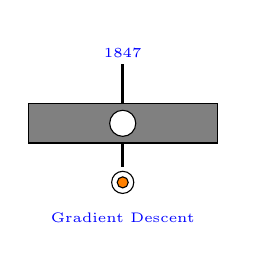
\begin{tikzpicture}[datemarker/.style={circle, draw=black,fill=white},textlabel/.style={anchor=center,text height=1.7ex,text depth=.25ex}]
					\tikzset{every node/.style={font=\tiny, color=blue}}\draw[fill=gray](-0.2,0) rectangle (2.2,0.5) node[white, below]{};
					\onslide<8->{\node at (1.0, 0.25) [datemarker] {};}
					\onslide<8->{\draw [line width=1pt] (1.0, 0.5) to (1.0, 1.0);}
					\onslide<8->{\draw (1.0, 1.2) node [textlabel] {1847 };}
					\onslide<8->{\draw [fill=orange](1.0, -0.5) circle (2pt){};}
					\onslide<8->{\draw (1.0, -0.5) circle (4pt){};}
					\onslide<8->{\draw [line width=1pt] (1.0, 0) to (1.0, -0.3);}
					\onslide<8->{\draw (1.0,-0.9) node [textlabel] {Gradient Descent};}
				\end{tikzpicture}
			\end{overlayarea}
			\column{0.9\textwidth}
			\begin{overlayarea}{\textwidth}{\textheight}
				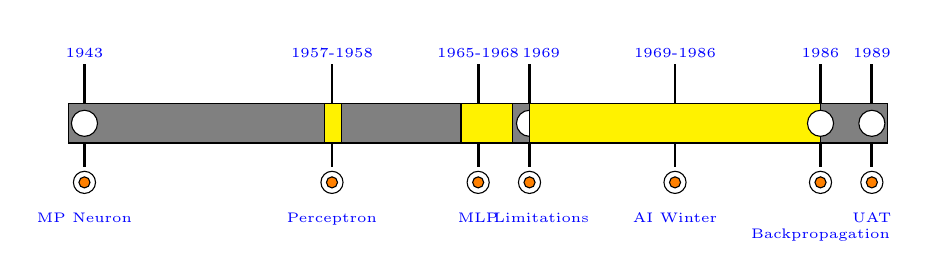
\begin{tikzpicture}[datemarker/.style={circle, draw=black,fill=white},textlabel/.style={anchor=center,text height=1.7ex,text depth=.25ex}]
					\tikzset{every node/.style={font=\tiny, color=blue}}\draw[fill=gray](-0.2,0) rectangle (10.2,0.5) node[white, below]{};
					\onslide<1->{\node at (0.0, 0.25) [datemarker] {};}
					\onslide<1->{\draw [line width=1pt] (0.0, 0.5) to (0.0, 1.0);}
					\onslide<1->{\draw (0.0, 1.2) node [textlabel] {1943 };}
					\onslide<1->{\draw [fill=orange](0.0, -0.5) circle (2pt){};}
					\onslide<1->{\draw (0.0, -0.5) circle (4pt){};}
					\onslide<1->{\draw [line width=1pt] (0.0, 0) to (0.0, -0.3);}
					\onslide<1->{\draw (0.0,-0.9) node [textlabel] {MP Neuron};}

					\onslide<2->{\draw[fill=yellow](3.04347826087, 0) rectangle (3.26086956522, 0.5){};}
					\onslide<2->{\draw [line width=1pt] (3.14347826087, 0.5) to (3.14347826087, 1.0);}
					\onslide<2->{\draw (3.14347826087, 1.2) node [textlabel] {1957-1958 };}
					\onslide<2->{\draw [fill=orange](3.14347826087, -0.5) circle (2pt){};}
					\onslide<2->{\draw (3.14347826087, -0.5) circle (4pt){};}
					\onslide<2->{\draw [line width=1pt] (3.14347826087, 0) to (3.14347826087, -0.3);}
					\onslide<2->{\draw (3.14347826087,-0.9) node [textlabel] {Perceptron};}


					\onslide<4->{\draw[fill=yellow](4.78260869565, 0) rectangle (5.4347826087, 0.5){};}
					\onslide<4->{\draw [line width=1pt] (5.0, 0.5) to (5.0, 1.0);}
					\onslide<4->{\draw (5.0, 1.2) node [textlabel] {1965-1968 };}
					\onslide<4->{\draw [fill=orange](5.0, -0.5) circle (2pt){};}
					\onslide<4->{\draw (5.0, -0.5) circle (4pt){};}
					\onslide<4->{\draw [line width=1pt] (5.0, 0) to (5.0, -0.3);}
					\onslide<4->{\draw (5.0,-0.9) node [textlabel] {MLP};}


					\onslide<5->{\node at (5.65217391304, 0.25) [datemarker] {};}
					\onslide<5->{\draw [line width=1pt] (5.65217391304, 0.5) to (5.65217391304, 1.0);}
					\onslide<5->{\draw (5.80217391304, 1.2) node [textlabel] {1969 };}
					\onslide<5->{\draw [fill=orange](5.65217391304, -0.5) circle (2pt){};}
					\onslide<5->{\draw (5.65217391304, -0.5) circle (4pt){};}
					\onslide<5->{\draw [line width=1pt] (5.65217391304, 0) to (5.65217391304, -0.3);}
					\onslide<5->{\draw (5.80217391304,-0.9) node [textlabel] {Limitations};}

					\onslide<6->{\draw[fill=yellow](5.65217391304, 0) rectangle (9.34782608696, 0.5){};}
					\onslide<6->{\draw [line width=1pt] (7.5, 0.5) to (7.5, 1.0);}
					\onslide<6->{\draw (7.5, 1.2) node [textlabel] {1969-1986};}
					\onslide<6->{\draw [fill=orange](7.5, -0.5) circle (2pt){};}
					\onslide<6->{\draw (7.5, -0.5) circle (4pt){};}
					\onslide<6->{\draw [line width=1pt] (7.5, 0) to (7.5, -0.3);}
					\onslide<6->{\draw (7.5,-0.9) node [textlabel] {AI Winter};}

					\onslide<7->{\node at (9.34782608696, 0.25) [datemarker] {};}
					\onslide<7->{\draw [line width=1pt] (9.34782608696, 0.5) to (9.34782608696, 1.0);}
					\onslide<7->{\draw (9.34782608696, 1.2) node [textlabel] {1986 };}
					\onslide<7->{\draw [fill=orange](9.34782608696, -0.5) circle (2pt){};}
					\onslide<7->{\draw (9.34782608696, -0.5) circle (4pt){};}
					\onslide<7->{\draw [line width=1pt] (9.34782608696, 0) to (9.34782608696, -0.3);}
					\onslide<7->{\draw (9.34782608696,-1.1) node [textlabel] {Backpropagation};}

					\onslide<9->{\node at (10.0, 0.25) [datemarker] {};}
					\onslide<9->{\draw [line width=1pt] (10.0, 0.5) to (10.0, 1.0);}
					\onslide<9->{\draw (10.0, 1.2) node [textlabel] {1989 };}
					\onslide<9->{\draw [fill=orange](10.0, -0.5) circle (2pt){};}
					\onslide<9->{\draw (10.0, -0.5) circle (4pt){};}
					\onslide<9->{\draw [line width=1pt] (10.0, 0) to (10.0, -0.3);}
					\onslide<9->{\draw (10.0,-0.9) node [textlabel] {UAT};}
				\end{tikzpicture}
			\end{overlayarea}
		\end{columns}
	\end{minipage}
\end{frame}


\makeatother
%	\author{Mitesh M. Khapra}
\title{Module 3}
\subtitle{The Deep Revival}
\author{}
\institute{}
\date{}
%\institute{Department of Computer Science and Engineering\\ Indian Institute of Technology Madras}
%\titlegraphic{\includegraphics[height=1cm,width=2cm]{images/iitm_logo.png}}
%\titlegraphicii{\includegraphics[height=1cm,width=2cm]{logo2}}

\begin{frame}
	\myheading{Chapter 3: The Deep Revival}
\end{frame}

\begin{frame}
	\begin{minipage}[t][0.6\textheight][t]{\textwidth}
		\begin{columns}
			\column{0.5\textwidth}
			\begin{overlayarea}{\textwidth}{\textheight}
				\justify
				\only<1>{\myheading{Unsupervised Pre-Training}}
				\only<1>{Hinton and  Salakhutdinov described an effective way of initializing the weights that allows deep autoencoder networks to learn a low-dimensional representation of data. \cite{Salakhutdinov:2012:ELP:2330716.2330717}}
			\end{overlayarea}
			\column{0.5\textwidth}
			\begin{overlayarea}{\textwidth}{\textheight}
				\begin{figure}
					\centering
					\only<1>{\includegraphics[scale=0.7]{"images/module3/2006_1"}}
				\end{figure}
			\end{overlayarea}
		\end{columns}
	\end{minipage}
	\begin{minipage}[t][0.4\textheight][t]{\textwidth}
		\begin{columns}
			\column{0.1\textwidth}
			\column{0.9\textwidth}
			\begin{overlayarea}{\textwidth}{\textheight}
				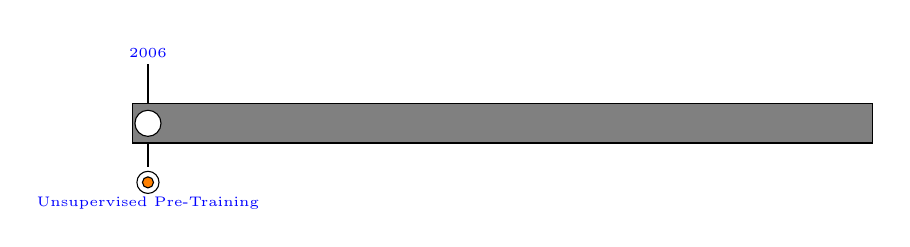
\begin{tikzpicture}[datemarker/.style={circle, draw=black,fill=white},textlabel/.style={anchor=center,text height=1.7ex,text depth=.25ex}]
					\tikzset{every node/.style={font=\tiny, color=blue}}\draw[fill=gray](-0.2,0) rectangle (9.2,0.5) node[white, below]{};
					\onslide<1>{\node at (0.0, 0.25) [datemarker] {};}
					\onslide<1>{\draw [line width=1pt] (0.0, 0.5) to (0.0, 1.0);}
					\onslide<1>{\draw (0.0, 1.2) node [textlabel] {2006 };}
					\onslide<1>{\draw [fill=orange](0.0, -0.5) circle (2pt){};}
					\onslide<1>{\draw (0.0, -0.5) circle (4pt){};}
					\onslide<1>{\draw [line width=1pt] (0.0, 0) to (0.0, -0.3);}
					\onslide<1>{\draw (0.0,-0.7) node [textlabel] {Unsupervised Pre-Training};}
				\end{tikzpicture}
			\end{overlayarea}
		\end{columns}
	\end{minipage}
\end{frame}
\begin{frame}
	\begin{minipage}[t][0.6\textheight][t]{\textwidth}
		\begin{columns}
			\column{0.5\textwidth}
			\begin{overlayarea}{\textwidth}{\textheight}
				\justify
				\only<1>{\myheading{Unsupervised Pre-Training}}
				\only<1>{The idea of unsupervised pre-training actually dates back to 1991-1993 (J. Schmidhuber) when it was used to train a ``Very Deep Learner''}
				\only<2>{\myheading{More insights (2007-2009)}}
				\only<2>{Further Investigations into the effectiveness of Unsupervised Pre-training}

				\only<3>{\myheading{Success in Handwriting Recognition}}
				\only<4>{\myheading{Success in Speech Recognition}}
				\only<5>{\myheading{ New record on MNIST }}
				\only<6>{\myheading{ First Superhuman Visual Pattern Recognition}}
				\only<7->{\myheading{Winning more visual recognition challenges}}

				\only<3>{Graves et. al. outperformed all entries in an international Arabic recognition competition \cite{NIPS2008_3449}}
				\only<4>{Dahl et. al. showed relative error reduction of 16.0\% and 23.2\% over a state of the art system \cite{Dahl:2012:CPD:2335874.2336015}}
				\only<5>{Ciresan et. al. set a new record on the MNIST dataset using good old backpropagation on GPUs (GPUs enter the scene)\cite{DBLP:journals/corr/abs-1003-0358}}
				\only<6>{D. C. Ciresan et. al. achieved 0.56\% error rate in the IJCNN Traffic Sign Recognition Competition \cite{DBLP:journals/corr/abs-1202-2745}}
				\only<7->{\begin{table}
						\begin{tabular}{ccc}
							\textbf{Network}                                                     & \textbf{Error}       & \textbf{Layers}      \\
							\onslide<7->{AlexNet \cite{NIPS2012_4824}}                           & \onslide<7->{16.0\%} & \onslide<7->{8}      \\
							\onslide<8->{ZFNet \cite{DBLP:journals/corr/ZeilerF13}}              & \onslide<8->{11.2\%} & \onslide<8->{8}      \\
							\onslide<9->{VGGNet \cite{DBLP:journals/corr/SimonyanZ14a}}          & \onslide<9->{7.3\%}  & \onslide<9->{19}     \\
							\onslide<10->{GoogLeNet \cite{DBLP:journals/corr/SzegedyLJSRAEVR14}} & \onslide<10->{6.7\%} & \onslide<10->{22}    \\
							\onslide<11->{MS ResNet \cite{DBLP:journals/corr/HeZRS15}}           & \onslide<11->{3.6\%} & \onslide<11->{152!!} \\
						\end{tabular}
					\end{table}
				}




			\end{overlayarea}
			\column{0.5\textwidth}
			\begin{overlayarea}{\textwidth}{\textheight}
				\begin{figure}
					\centering
					\only<1>{\includegraphics[scale=0.7]{"images/module3/2006_1"}}
					\only<2>{\includegraphics[scale=0.23]{"images/module3/2007"}}
					\only<3>{\includegraphics[scale=0.15]{"images/module3/2009"}}
					\only<4>{\includegraphics[scale=0.5]{"images/module3/2010_1"}}
					\only<5>{\includegraphics[scale=0.5]{"images/module3/2010"}}
					\only<6>{\includegraphics[scale=0.4]{"images/module3/2011"}}
					\only<7->{\includegraphics[scale=0.4]{"images/module3/2012_1"}}


				\end{figure}
			\end{overlayarea}
		\end{columns}
	\end{minipage}
	\begin{minipage}[t][0.4\textheight][t]{\textwidth}
		\begin{columns}
			\column{0.1\textwidth}
			\begin{overlayarea}{\textwidth}{\textheight}
				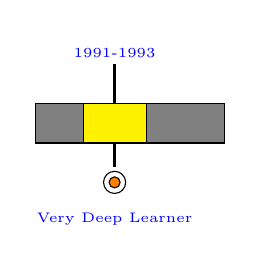
\begin{tikzpicture}[datemarker/.style={circle, draw=black,fill=white},textlabel/.style={anchor=center,text height=1.7ex,text depth=.25ex}]
					\tikzset{every node/.style={font=\tiny, color=blue}}\draw[fill=gray](-0.2,0) rectangle (2.2,0.5) node[white, below]{};

					\onslide<1->{\draw[fill=yellow] (0.4, 0) rectangle (1.2, 0.5){};}
					\onslide<1->{\draw [line width=1pt] (0.8, 0.5) to (0.8, 1.0);}
					\onslide<1->{\draw (0.8, 1.2) node [textlabel] {1991-1993 };}
					\onslide<1->{\draw [fill=orange](0.8, -0.5) circle (2pt){};}
					\onslide<1->{\draw (0.8, -0.5) circle (4pt){};}
					\onslide<1->{\draw [line width=1pt] (0.8, 0) to (0.8, -0.3);}
					\onslide<1->{\draw (0.8,-0.9) node [textlabel] {Very Deep Learner};}
				\end{tikzpicture}
			\end{overlayarea}


			\column{0.9\textwidth}
			\begin{overlayarea}{\textwidth}{\textheight}
				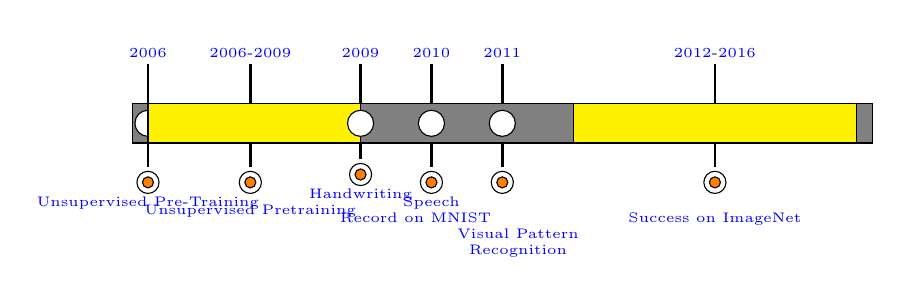
\begin{tikzpicture}[datemarker/.style={circle, draw=black,fill=white},textlabel/.style={anchor=center,text height=1.7ex,text depth=.25ex}]
					\tikzset{every node/.style={font=\tiny, color=blue}}\draw[fill=gray](-0.2,0) rectangle (9.2,0.5) node[white, below]{};
					\onslide<1>{\node at (0.0, 0.25) [datemarker] {};}
					\onslide<1>{\draw [line width=1pt] (0.0, 0.5) to (0.0, 1.0);}
					\onslide<1>{\draw (0.0, 1.2) node [textlabel] {2006 };}
					\onslide<1>{\draw [fill=orange](0.0, -0.5) circle (2pt){};}
					\onslide<1>{\draw (0.0, -0.5) circle (4pt){};}
					\onslide<1>{\draw [line width=1pt] (0.0, 0) to (0.0, -0.3);}
					\onslide<1>{\draw (0.0,-0.7) node [textlabel] {Unsupervised Pre-Training};}

					\onslide<2->{\draw [fill=yellow] (0,0) rectangle (2.7, 0.5){};}
					\onslide<2->{\draw [line width=1pt] (1.3, 0.5) to (1.3, 1.0);}
					\onslide<2->{\draw (1.3, 1.2) node [textlabel] {2006-2009};}
					\onslide<2->{\draw [fill=orange](1.3, -0.5) circle (2pt){};}
					\onslide<2->{\draw (1.3, -0.5) circle (4pt){};}
					\onslide<2->{\draw [line width=1pt] (1.3, 0) to (1.3, -0.3);}
					\onslide<2->{\draw (1.3,-0.8) node [textlabel] {Unsupervised Pretraining};}


					\onslide<3->{\node at (2.7, 0.25) [datemarker] {};}
					\onslide<3->{\draw [line width=1pt] (2.7, 0.5) to (2.7, 1.0);}
					\onslide<3->{\draw (2.7, 1.2) node [textlabel] {2009 };}
					\onslide<3->{\draw [fill=orange](2.7, -0.4) circle (2pt){};}
					\onslide<3->{\draw (2.7, -0.4) circle (4pt){};}
					\onslide<3->{\draw [line width=1pt] (2.7, 0) to (2.7, -0.2);}
					\onslide<3->{\draw (2.7,-0.6) node [textlabel] {Handwriting};}

					\onslide<4->{\node at (3.6, 0.25) [datemarker] {};}
					\onslide<4->{\draw [line width=1pt] (3.6, 0.5) to (3.6, 1.0);}
					\onslide<4->{\draw (3.6, 1.2) node [textlabel] {2010 };}
					\onslide<4->{\draw [fill=orange](3.6, -0.5) circle (2pt){};}
					\onslide<4->{\draw (3.6, -0.5) circle (4pt){};}
					\onslide<4->{\draw [line width=1pt] (3.6, 0) to (3.6, -0.3);}
					\onslide<4->{\draw (3.6,-0.7) node [textlabel] {Speech};}

					\onslide<5->{\draw (3.4,-0.9) node [textlabel] {Record on MNIST};}

					\onslide<6->{\node at (4.5, 0.25) [datemarker] {};}
					\onslide<6->{\draw [line width=1pt] (4.5, 0.5) to (4.5, 1.0);}
					\onslide<6->{\draw (4.5, 1.2) node [textlabel] {2011 };}
					\onslide<6->{\draw [fill=orange](4.5, -0.5) circle (2pt){};}
					\onslide<6->{\draw (4.5, -0.5) circle (4pt){};}
					\onslide<6->{\draw [line width=1pt] (4.5, 0) to (4.5, -0.3);}
					\onslide<6->{\draw (4.7,-1.1) node [textlabel] {Visual Pattern};}
					\onslide<6->{\draw (4.7,-1.3) node [textlabel] {Recognition};}


					\onslide<7->{\draw [fill=yellow] (5.4,0) rectangle (9.0, 0.5){};}
					\onslide<7->{\draw [line width=1pt] (7.2, 0.5) to (7.2, 1.0);}
					\onslide<7->{\draw (7.2, 1.2) node [textlabel] {2012-2016 };}
					\onslide<7->{\draw [fill=orange](7.2, -0.5) circle (2pt){};}
					\onslide<7->{\draw (7.2, -0.5) circle (4pt){};}
					\onslide<7->{\draw [line width=1pt] (7.2, 0) to (7.2, -0.3);}
					\onslide<7->{\draw (7.2,-0.9) node [textlabel] {Success on ImageNet};}
				\end{tikzpicture}
			\end{overlayarea}
		\end{columns}
	\end{minipage}
\end{frame}

\include{modules/Module4/Lecture1_4}

\include{modules/Module5/Lecture1_5}

\include{modules/Module6/Lecture1_6}

\include{modules/Module7/Lecture1_7}

\include{modules/Module8/Lecture1_8}

\makeatother
%	\author{Mitesh M. Khapra}
\title{Module 9}
\subtitle{(Need for) Sanity}
\author{}
\institute{}
\date{}
%\institute{Department of Computer Science and Engineering\\ Indian Institute of Technology Madras}
%\titlegraphic{\includegraphics[height=1cm,width=2cm]{images/iitm_logo.png}}
%\titlegraphicii{\includegraphics[height=1cm,width=2cm]{logo2}}
\renewcommand{\thefootnote}{\roman{footnote}}
\begin{frame}
	\myheading{Chapter 9: (Need for) Sanity}
\end{frame}
\begin{frame}
	\begin{columns}
		\column{0.55\textwidth}
		\begin{overlayarea}{\textwidth}{\textheight}
			\footnotesize{
				\justify
				\myheading{The Paradox of Deep Learning}
				Why does deep learning work so well despite
				\begin{itemize}
					\item<2-> {high capacity (susceptible to overfitting)}
					\item<3-> {numerical instability (vanishing/exploding gradients)}
					\item<4-> {sharp minima (leading to overfitting)}
					\item<5-> {non-robustness (see figure)}
				\end{itemize}
				~\\
				\only<6->{No clear answers yet but ...}
				\begin{itemize} \justifying
					\item<7->{Slowly but steadily there is increasing emphasis on explainability and theoretical justifications!$^*$ \footnotetext{$^*$\url{https://arxiv.org/pdf/1710.05468.pdf}}}
					\item<8->{ Hopefully this will bring sanity to the proceedings !}
				\end{itemize}}
		\end{overlayarea}
		\column{0.45\textwidth}
		\begin{overlayarea}{\textwidth}{\textheight}
			\begin{figure}
				\centering
				\vspace{0.2in}
				\only<1->{\includegraphics[scale=0.4]{"images/module9/adversarial_img_1"}}
			\end{figure}
		\end{overlayarea}
	\end{columns}
\end{frame}



\begin{frame}
	\centering
	\small{\url{https://github.com/kjw0612/awesome-rnn}}
\end{frame}

\begin{frame}
	\begin{figure}[ht]
		\centering
		\fcolorbox{black}{gray}{\includegraphics[width=1\linewidth]{images/Deep_learning_MarketMap_sept2016_featured}}
		%      \label{fig:startups}
		%      \caption*{The Deep Learning Market Map}

	\end{figure}
	\footnotetext[1]{Source: https://www.cbinsights.com/blog/deep-learning-ai-startups-market-map-company-list/}
\end{frame}



\begin{frame}[allowframebreaks]{References}
	\nocite{*}
	\tiny
	\bibliographystyle{unsrt}
	\bibliography{ref}


\end{frame}
\end{document}
